%%%%%%%%%%%%%%%%%%%%%%%%%%%%%%%%%%%%%%%%%%%%%%%%%%%%%%%%%%%%%%%%%%
%%%%%%%% ICML 2013 EXAMPLE LATEX SUBMISSION FILE %%%%%%%%%%%%%%%%%
%%%%%%%%%%%%%%%%%%%%%%%%%%%%%%%%%%%%%%%%%%%%%%%%%%%%%%%%%%%%%%%%%%

% Use the following line _only_ if you're still using LaTeX 2.09.
%\documentstyle[icml2013,epsf,natbib]{article}
% If you rely on Latex2e packages, like most moden people use this:
\documentclass{article}

% For figures
\usepackage{graphicx} % more modern
%\usepackage{epsfig} % less modern
\usepackage{subfigure} 

% For citations
\usepackage{natbib}

% For math
\usepackage{array}
\usepackage{amssymb}
\usepackage{amsmath}
\usepackage{amsthm}

% For algorithms
\usepackage{algorithm}
\usepackage{algorithmic}

% As of 2011, we use the hyperref package to produce hyperlinks in the
% resulting PDF.  If this breaks your system, please commend out the
% following usepackage line and replace \usepackage{icml2013} with
% \usepackage[nohyperref]{icml2013} above.
\usepackage{hyperref}

% Packages hyperref and algorithmic misbehave sometimes.  We can fix
% this with the following command.
\newcommand{\theHalgorithm}{\arabic{algorithm}}

\DeclareMathOperator*{\argmax}{arg\,max}

% Employ the following version of the ``usepackage'' statement for
% submitting the draft version of the paper for review.  This will set
% the note in the first column to ``Under review.  Do not distribute.''
% \usepackage{icml2013} 
% Employ this version of the ``usepackage'' statement after the paper has
% been accepted, when creating the final version.  This will set the
% note in the first column to ``Proceedings of the...''
\usepackage[accepted]{icml2013}


% The \icmltitle you define below is probably too long as a header.
% Therefore, a short form for the running title is supplied here:
\icmltitlerunning{Deep Belief Networks for Audio Chord Recognition}

\begin{document} 

\twocolumn[
\icmltitle{Deep Belief Networks for Audio Chord Recognition}

% It is OKAY to include author information, even for blind
% submissions: the style file will automatically remove it for you
% unless you've provided the [accepted] option to the icml2013
% package.
\icmlauthor{Benjamin Rapaport}{bar2150@columbia.edu}
\icmladdress{Columbia University,
            2960 Broadway  New York, NY 10027}
\icmlauthor{Samuel Messing}{sbm2158@columbia.edu}
\icmladdress{Columbia University,
            2960 Broadway  New York, NY 10027}

% You may provide any keywords that you 
% find helpful for describing your paper; these are used to populate 
% the "keywords" metadata in the PDF but will not be shown in the document
\icmlkeywords{deep learning, deep belief networks, hessian free, machine learning}

\vskip 0.3in
]

\begin{abstract}

Feature selection plays a critical role in audio analysis, with most Music
Information Retrieval (MIR) systems relying on a standard set of manually
crafted domain-specific features sets. In this paper, we survey a number of
methods related to training and constructing Deep Belief Networks in order to
perform unsupervised feature learning as well as classification in order t
recognize chord sequences in audio signals. Specifically, we train deep neural
networks using the contrastive divergence unsupervised method, supervised
backpropogation optimization, as well as supervised Hessian Free optimization
techniques. The activations of these networks are then fed into a structured
support vector machine (SVMStruct) in order to make chord predictions over
entire song sequences.

TODO(ben): what were our general results?

\end{abstract} 

\section{Introduction}

The success and failure of many machine learning techniques is often
strongly influenced by the representations of the data used for learning.
Historically, this has meant that a lot of effort has gone into feature
engineering, where domain-specific expertise and human enginuity have been
used to manually craft a set of preprocessing steps in order to get the data
into a proper format for the learning task at hand. However, more recently,
the field of automated feature learning, or deep learning, has shown that
more general methods can be used to preprocess data and lead to highly effective
and often state-of-the-art learning performance.

One of the most popular and successful methods for feature selection has been
to use Deep Belief Networks (DBN) to learn a set of features that can then
be used for classification tasks. This technique has been used to achieve
state-of-the-art performance on a number of standard learning tasks across
multiple mediums. These include tasks in speech recognition 
\cite{Mohamed_acousticmodeling, dahl2010phone}, polyphonic music transciption
\cite{boulanger2012modeling}, and object recognition 
\cite{krizhevsky2012imagenet, ciresan2012multi, rifai2011manifold}, among
others.

Deep Belief Networks are a type of deep neural network that has multiple hidden
layers. Recent advances in training these deep networks has shown that they are
capable of learning highly complex non-linear representations of their input.
It has been shown that these these networks model their inputs such that each
hidden layer captures information at a potentially higher level of abstraction
than the one below it \cite{Bengio_learning}. 

In this work, we investigate using deep architectures, specifically
Deep Belief Networks (DBN) in order to
TODO(ben): finish intro

\section{Dataset} 
The training and evaluation of our techniques were performed over a set of 180
hand-labeled Beatles songs \cite{harte2010towards}. The set of chord labels
was restricted to just the triads, 12 for major triads, 12 for minor triads,
and a final label representing 'no chord', leading to a total of 25 possible
chord labels.

\subsection{Chroma}
The labeled data was offered in the Chroma format, in which a song is split into
beat-synchronous frames, each containing 12 features that represent the
intensity of each semitone, irrespective of octave. Each of these features
is constrained to be in the range [0,1].

\subsection{Short Time Fourier Transform}
We also took the raw audio data for the songs 
TODO(SAM): Can you describe how we did this part? Window size, sampling rates,
DFTs, absolute values, final input dimension, etc.

\section{Deep Belief Networks}

\begin{figure}[ht]
\vskip 0.2in
\begin{center}
\centerline{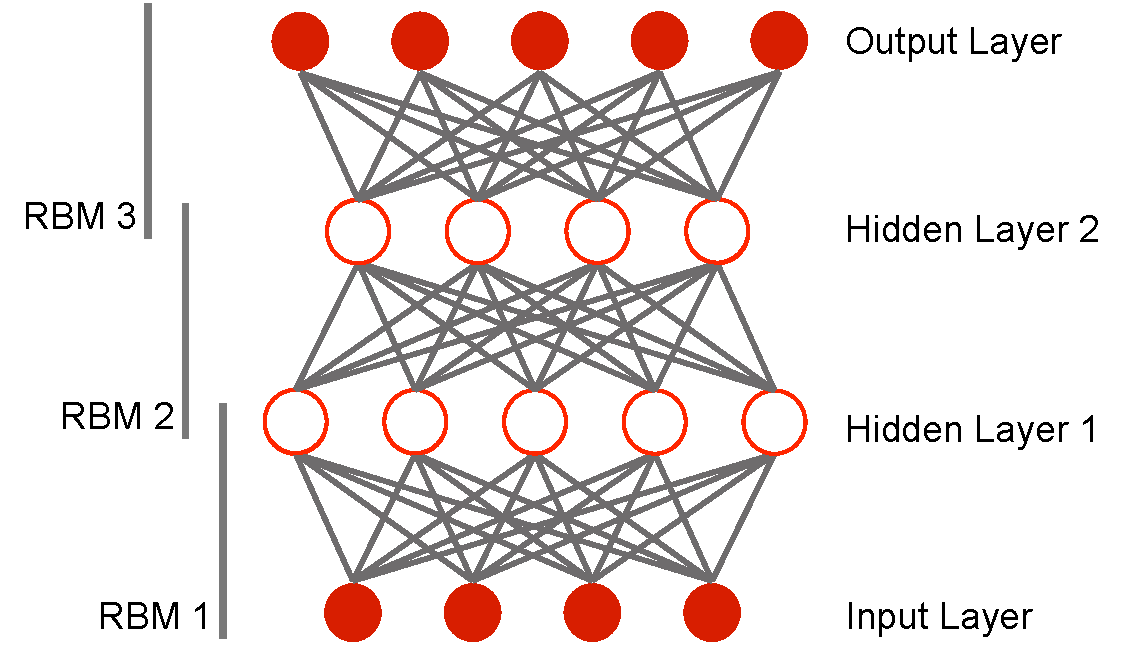
\includegraphics[width=\columnwidth]{images/deep_network_arch.pdf}}
\caption{The general architecture of a DBN as a series of stacked RBMs}
\label{dbn-arch}
\end{center}
\vskip -0.2in
\end{figure}

\subsection{Restricted Boltzmann Machines}

The main building block of a Deep Belief Network is the Restricted Boltzmann
Machine (RBM). An RBM is an undirected graphical model that represents a
generative joint probability distribution over a visible vector $\mathbf{v}$
and a hidden vector $\mathbf{h}$ \cite{mnih2012conditional}. The RBM forms a
bipartite graph, where each visible node is connected to every hidden node, but
is not connected to any other visible nodes, and vice versa for the hidden
nodes.  This allows for a nice factorization of the conditional probability
distributions, and allows for efficient computation without worrying about the
'explaining away' phenomenon. Assuming each of these vectors is binary,
the RBM models the joint probability distribution

\[
  p \left( \mathbf{v}, \mathbf{h} \right) = 
  exp \left(-E \left( \mathbf{v}, \mathbf{h} \right) \right) / Z,
\]

where $Z$ is the normalization term, and $E$ is an energy function defined as

\[
  E \left( \mathbf{v}, \mathbf{h} \right) = 
  - \mathbf{v^TWh} - \mathbf{v^Tb^v} - \mathbf{h^Tb^h}.
\]

$\mathbf{W}$ is a matrix of pairwise weights between the elements in 
$\mathbf{v}$ and $\mathbf{h}$, $\mathbf{b^v}$ are the biases for the visible
vector elements, and $\mathbf{b^h}$ are the biases for the hidden vector
elements.

If we define the free energy $F(\mathbf{v})$ as
\begin{align*}
  F \left( \mathbf{v} \right) &= -log \sum_{\mathbf{h}} exp \left( -E \left( \mathbf{v,h} \right) \right) \\
  &= \mathbf{v^Tb^v} - \sum_{\mathbf{j}} log
    \left(
      1 + exp \left( b_j^h + \mathbf{v^TW_{\cdot j}} \right)
    \right), \\
\end{align*}

then we can obtain the distribution $p(\mathbf{v})$ by marginalizing over
$\mathbf{h}$

\begin{align*}
  p(\mathbf{v}) &= \sum_{\mathbf{h}} exp(-E(\mathbf{v, h})) / Z \\
                &= exp(-F(\mathbf{v})) / Z. \\
\end{align*}

An RBM can then be trained using gradient descent of the negative
log-likelihood, where the log-likelihood is defined as:

\begin{align*}
  l(\theta) &= log \, p(\mathbf{v}) \\
            &= -F(\mathbf{v}) - log \sum_{\mathbf{v'}} exp (-F(\mathbf{v'})), \\
\end{align*}

and the gradient

\[
  \frac{- \partial l(\theta)}{\partial \theta}
  = \frac{\partial F(\mathbf{v})}{\partial \theta} - 
  \sum_{\mathbf{v'}}\frac{\partial F(\mathbf{v'})}{\partial \theta}
                  p(\mathbf{v})
\]


\subsection{Contrastive Divergence}

The gradient described prevously cannot be computed tractably for large models,
as it requires computing an expectation over the model distribution
$p(\mathbf{v})$.  However, we can still train RBMs efficiently using a
technique introduced by Hinton called Contrastive Divergence
\cite{hinton_contrastivedivergence}. The derivative of the log probability of a
training vector with respect to a weight in $\mathbf{W}$ is 

\[
  \frac{\partial log p(\mathbf{v})}{\partial w_{ij}} = 
  \langle v_i h_j \rangle_{data} - \langle v_i h_j \rangle_{model}
\]

where the angle brackets indicate expectaions under the specified distributions.
Because the RBM is bipartite, obtaining samples from the hidden units given
visible activations is simply

\[
  p (h_j = 1 | \mathbf{v}) = \sigma(b_{j}^{h} + \sum_i v_{i} w_{ij})
\]

and obtaining samples for the visible units given hidden activations is
\[
  p (v_i = 1 | \mathbf{h}) = \sigma(b_{i}^{v} + \sum_j h_j w_{ij}).
\]

where $\sigma$ is the logistic sigmoid function.

If the visible units are real-valued, instead of binary, we can use a
Gaussian-Bernoulli RBM by simply changing the sampling equation for the visible
vector to be:
\[
  p (v_i | \mathbf{h}) = \mathcal{N} \left( b_{i}^{v} +
    \sigma_i \sum_j h_j w_{ij} \,,\, \sigma_i^2 \right),
\]

where we generally normalize the data such that $\sigma = 1$.

We could compute the expectation under the model by running a Gibbs chain for a
long time, where we alternatively sample hidden states given visible states,
and visible states given hidden states repeatedly until we converged on the
model distribution. However, the insight of Contrastive Divergence is that if
we initialize the visible vector by clamping it to a training vector sampled
from the empirical data distribution, and only take a few Gibbs sampling steps,
we can obtain an estimate of the model distribution called the
``reconstruction'' that works well empirically for estimating the gradient. In
fact, good results can be obtained by simply taking a single Gibbs step to
create this reconstruction. The learning rule for updating a weight between two
units with learning rate $\epsilon$ is then

\[
  \triangle w_{ij} = \epsilon( 
  \langle v_i h_j \rangle_{data} - \langle v_i h_j \rangle_{recon}
  )
\]
which can be computed very efficiently.

\subsection{Training a DBN with Constrastive Divergence and Supervised Fine Tuning}

By stacking a series of RBMs, we can use this Constrastive Divergence technique
to train each RBM separately in a greedy, layer-wise fashion in order to train
a deep architecture. With these stacked RBMs, the hidden layer of one RBM
becomes the visible layer of the RBM above it, and each is trained by sampling
from the distributions below it to initiate the visible vectors for
Contrastive Divergence training.

Once each layer has been trained, the final step for training the DBN is to
unfold its layers into a standard, feed-forward neural network, and add a final
softmax layer of output units that we can use for classification. We use the
weights learned from the unsupervised Contrastive Divergence pretraining to
then initialize this feed forward network, which we can train in a supervised
manner using standard backpropogation on a set of labeled examples. In this
manner we allow the unsupervised phase to find a good initialization of the
weights by potentially avoiding local minima, and let the supervised
backpropogation training ``fine-tune'' the model to perform well on the
classification task at hand.

\subsection{Training a Deep Neural Network with Hessian Free Optimization}

Hessian-Free optimization (HF) techniques belong to the class of approximate
Newton methods for the minimization of real-valued smooth objective functions
\cite{martens2012training}. In 2010, Martens introduced an algorithm for
training deep neural networks using Hessian-Free optimization on only labeled
data, without the need for unsupervised pre-training \cite{martens2010deep}.
Using HF, Martens was able to obtain similar or even superior results for
training deep networks than the standard methods described above. 

The basic idea behind HF is derived from the classical Newton's method, where
local quadratic approximations of the objective function are iteratively
optimized to produce updates to the parameters $\mathbf{\theta}$.  More
precisely, at each step we optimize a local quadratic model
$M_{k-1}(\mathbf{\delta)}$ of the objective function $f(\mathbf{\theta_{k-1}} +
\mathbf{\delta})$ which is estimated using the gradient and curvature
information local to $\mathbf{\theta_{k-1}}$ to produce a new parameter vector
$\mathbf{\theta_k}$. The quadratic approximation is defined as

\[
  M_{k-1}(\mathbf{\delta}) = f(\mathbf{\theta}_{k-1})
  + \nabla f(\mathbf{\theta_{k-1})^T \delta}
  + \frac{1}{2} \mathbf{\delta^T B_{k-1} \delta}
\]

where $\mathbf{B_{k-1}}$ is the curvature matrix, which is the Hessian
$\mathbf{H(\theta_{k-1})}$ of $f$ at $\mathbf{\theta_{k-1}}$ for the standard
Newton's method. The updated parameters are then computed as
$\mathbf{\theta_{k=1}} + \alpha_k \mathbf{\delta^{*}_{k}}$, where
$\mathbf{\delta^{*}_{k}}$ is the minimizer of $M_{k-1}(\mathbf{\delta)}$ and
$\alpha_k$ is a step-size chosen via a line-search.

When the curvature matrix $\mathbf{B_{k-1}}$ is positive definite, the minimizer will
exist and is given by

\[
  \mathbf{\delta^{*}_{k}} =
  \mathbf{\theta_k} - \mathbf{B^{-1}_{k-1}} \nabla f(\mathbf{\theta_{k-1}}).
\]

However, using the Hessian as the curvature matrix makes this computation
generally intractible as the Hessian itself is quadratic in the number
of parameters, which in the case of deep neural networks is very large.
Additionally, inverting the Hessian to solve for the minimizer has a computational
complexity of $O(n^3)$.

To avoid this computational cost of inversion, HF and other so-called
Truncated-Newton methods approximately optimize the quadratic function $M$
using the conjugate gradient algorithm in order to update $\theta$.

Conjugate Gradient has the additional property that it only requires the use
of matrix-vector products with the curvature matrix $\mathbf{B}$, which can
be computed more efficiently than the entire matrix.

In addition to providing a method to compute these matrix-vector products efficiently
in the case of a deep neural network, Martens also recommends using a generalized
Gauss-Newton matrix as the curvature matrix, as an estimation of the Hessian.
A nice property of this curvature matrix is that it does not have some of the
problems of indefiniteness that the true Hessian can have, which allows for 
optimization via conjugate gradient to proceed properly. 

For more details on this HF optimization method, we point the reader to
Marten's work on the subject \cite{martens2010deep}. However, it has been noted
that this method can be a more effective optimizer than normal gradient descent
methods such as backpropogation, since it can use information about the curvature
of the objective function to gauge its parameter updates. This may allow it
to avoid pathological curvature in the parameter space, which seems to be an
issue when training deep neural networks.

\section{Large Margin Structured Predictions}

Finally, to make predictions for the sequence of chord labels over a song,
we turn to an extension of Support Vector Machines (SVM) that can support
structured classification problems such as sequence prediction. Under this
extension, the goal is to learn a function $F : X \times Y \rightarrow
\mathbf{R}$ with weight vector $\mathbf{w}$ such that,

\begin{equation*}
f(\mathbf{x}) = \argmax_{y \in Y}F(\mathbf{x},\mathbf{y}\,;\,\mathbf{w})
\end{equation*}

correctly predicts the true label $y$. Given a series of $N$ data points
$(\mathbf{x}^{(i)}, \mathbf{y}^{(i)})_{i=1}^{N}$, we can learn the weight
vector $\mathbf{w}$ by imposing data-specific constraints of the following
form,

\begin{equation*}
\begin{split}
F(\mathbf{x}^{(i)}, \mathbf{y}^{(i)}\,;\,\mathbf{w}) -
F(\mathbf{x}^{(i)}, \mathbf{y}'\,;\,\mathbf{w}) \geq 1 \\
\forall i \in 1\dots N,\,\mathbf{y}' \neq \mathbf{y}^{(i)}
\end{split}
\end{equation*}

Learning is accomplished by minimizing $||\mathbf{w}||$ subject to the
data-specific constraints. The optimization problem is thus,

\[
\begin{split}
\min_{\mathbf{w}}\dfrac{1}{2}||\mathbf{w}||\quad\text{such that,} \\
F(\mathbf{x}^{(i)}, \mathbf{y}^{(i)}\,;\,\mathbf{w}) -
F(\mathbf{x}^{(i)}, \mathbf{y}'\,;\,\mathbf{w}) \geq 1 \\
\forall i \in 1\dots N, \,\mathbf{y}' \neq \mathbf{y}^{(i)}
\end{split}
\]

When data is non-separable, additional slack variables are introduced to allow
for a certain amount of disagreement between the predicted and true labels.
  This enables the learning algorithm to effectively ignore hard-to-label
  points. With the added $N$ slack variables, $\xi$, the optimization problem
  becomes,

\begin{align*}
\begin{split}
\min_{\mathbf{w, \xi}}\dfrac{1}{2}||\mathbf{w}|| +
\dfrac{C}{N}\sum_{i=1}^{N}\xi^{(i)}
\quad\text{such that,}&\\
F(\mathbf{x}^{(i)}, \mathbf{y}^{(i)}\,;\,\mathbf{w}) -
F(\mathbf{x}^{(i)}, \mathbf{y}'\,;\,\mathbf{w}) \geq 1 - \xi^{(i)} \\
\forall i \in 1\dots N, \,\mathbf{y}' \neq \mathbf{y}^{(i)}
\end{split}
\end{align*}

Where $C$ is a tuneable parameter that represents the cost associated with
using slack. When $C = \infty$, the optimization problem is the same as in
the separable case.

For sequence learning, the class $Y$ of possible labelings can be exponential
in size, and therefore it is often infeasible to enumerate all of the
data-specific constraints. Instead, the SVM$^{struct}$ algorithm uses an
efficient cutting-plane approach to find a solution after adding only a
polynomial number of constraints. This involves reformulating the problem from
an $N$-slack problem ($N$ $\xi$ variables) to a 1-slack problem (only a single
$\xi$ variable). This reformulation only requires that the calculation of
$\hat{y} = \argmax_{y \in Y}$ be efficiently computible for all examples. The
details can be found in \cite{joachims2009cutting}.

\subsection{The SVM$^{hmm}$ model}

The SVM$^{hmm}$ model is a particular formulation of SVM$^{struct}$ where the
disciminant function is constructed to be isomorphic to a $k$th order Hidden
Markov Model (HMM). This model was first described in
\cite{altun2003hidden}. While this model does not have the same
probabilistic interpretation as the HMM, by mimicking the structure of a
traditional HMM, $\argmax_{y \in Y}$ becomes efficient to compute, as the same
Markov property\footnote{Again, we stress that in the case of SVM$^{hmm}$ there
is no probabilistic interpetation, we use the term ``Markov property'' loosely.}
can be exploited, simplifying the algorithm. This enables the use of the
cutting-plane method mentioned above..

To mimic a $k$th order HMM, the function $F$ used by SVM$^{hmm}$ is of the
form,

\begin{flalign*}
  &{F(\mathbf{x}, \mathbf{y}\,;\,\mathbf{w})} =& \\
    & \sum_{t=1}^{T} \left[
      \sum_{k=1}^{K}\left(
        \mathbf{x}_{t} \cdot
        \mathbf{w}_{\mathbf{y}_{(t-k)} \dotsm \mathbf{y}_{t}} +
        \phi_{\text{trans}}(y_{(t-k)},\dots,y_{t}) \cdot
        \mathbf{w}_{\text{trans}}
      \right)
    \right]  &
\end{flalign*}

Where $T$ is the number of time frames in an individual example ($\mathbf{x}$,
$\mathbf{y}$), $x_t$ is the $t^{\text{th}}$ frame of example $x$, $K$ is the
order of dependencies, and $\phi_{\text{trans}}$ is an indicator vector that
has exactly one entry 'on' (equal to 1) and all others 'off' (equal to 0),
corresponding to the sequence $(y_{(t-k)},\dots,y_{t})$.

\section{Methods}

For all of our methods, we tried using the chroma as the inputs, as well
the raw STFTs. For the STFTs, we perform a PCA whitening step to the data
so that the input vectors have zero mean, and spherical identity variance. 
We would concatenate surrounding frames to the input vectors we want
to classify to give more contextual information to the algorithms.

We took the chosen inputs, and trained a deep network using either the
Contrastive Divergence unsupervised training followed by supervised
backpropogation, or by training the entire network in a supervised fashion
using the Hessian Free technique. For the Contrastive Divergence learning, we
made use of a library provided by Rasmus Berg Palm \cite{IMM2012-06284}. For
the HF technique, we used code provided by Martens \cite{martens2010deep}.

After training, the test data was then either classified directly by the output
layer of the trained discriminative network, or it was used to detmine network
activations which were then fed into the structured SVM classifier
\cite{joachims1999making}. For every experiment, 5 random permutations of the
songs were used for training, with 10\% of the total song corpus reserved for
training, and 10\% used as a validation set for when to stop the network
training. All results report the average of these 5 permutations.

For all SVM training, we set $epsilon$ to 1 and $C$ to 100. Additionally,
even when we trained the networks on 80\% of the data, we only trained the
SVM on 30\% of the data, due to computational costs.

\section{Results}

\bibliography{deep_belief_nets}
\bibliographystyle{icml2013}

\end{document} 


% This document was modified from the file originally made available by
% Pat Langley and Andrea Danyluk for ICML-2K. This version was
% created by Lise Getoor and Tobias Scheffer, it was slightly modified  
% from the 2010 version by Thorsten Joachims & Johannes Fuernkranz, 
% slightly modified from the 2009 version by Kiri Wagstaff and 
% Sam Roweis's 2008 version, which is slightly modified from 
% Prasad Tadepalli's 2007 version which is a lightly 
% changed version of the previous year's version by Andrew Moore, 
% which was in turn edited from those of Kristian Kersting and 
% Codrina Lauth. Alex Smola contributed to the algorithmic style files.  
